\documentclass[english,10pt,twocolumn]{article}

\usepackage{times}
\usepackage{fullpage}
\usepackage{babel}
\usepackage{graphicx}


\begin{document}

\title{A Unikernel Key-Value Store}
\author{Nate Brennand, Gudbergur Erlendsson, Mishail Tupas}
\date{}
\maketitle
\thispagestyle{empty}


\begin{abstract}
Traditional web infrastructure models consist of a cluster of heavyweight full stack virtual machines usually running a variant of Linux.
This provides a simple consistent platform for developers to write their applications against but it has many downfalls in the resource overhead of running virtual machines.
Key-value datastores are a common component of web insfrastructure.
<<<<<<< HEAD
We've designed a MirageOS\cite{mirage} unikernel implementation of the popular Redis\cite{redis} in-memory key-value store that allows fast creation and deployment of the datastore as well as ease scaling up the allocated resources.
Applications developed with MirageOS can be deployed directly on the Xen hypervisor.
=======
We've designed a Mirage OS\cite{mirage} unikernel implementation of the popular Redis\cite{redis} key-value store that allows fast creation and deployment of the datastore as well as ease scaling up the allocated resources.
>>>>>>> origin/evaluation
We describe the advantages and disadvantages that come with such a system.
We highlight the performance characteristics of this new approach in comparison to Redis.

Preliminary results show comparable performance.
We expect with more profiling we can identify the hotspots in our codebase and garner better performance from the Kayvee implementation.
\end{abstract}


\section{Introduction}
In-memory key-value datastores are used in a wide variety of applications for ease of use and the high throughput.
While these applications are known for their great performance, research has shown that networked applications striving for low latency, such as Redis, are actually subjected to a high amount of overhead from utilizing Linux's networking stack.\cite{arrakis}
This issue is amplified by the lack of stability in allocated resources when running on Linux itself which is prone to performance dips when the resource scheduler is not coordinated.

We believe that the approach of moving the key-value datastore to a unikernel implementation will yield greater and more reliable performance.
A unikernel is a specialzed application capable of running directly on top of bare-metal or a hypervisor without a host operating system.
The unikernel approach lacks many of the performance issues plaguing Redis that cannot be resolved at the application level.
<<<<<<< HEAD
We build on top of the MirageOS\cite{mirage}, an OCaml based library operating system.
MirageOS provides correctness due to the strongly-typed nature of OCaml, this yields very reliable code.
=======
We build on top of the Mirage OS\cite{mirage}, an OCaml based library operating system that provides type-safe networking libraries.
>>>>>>> origin/evaluation

We measure the performance characteristics of Redis in multiple situations: networked and on-host, to yield a direct comparison to our implementation, Kayvee.
Kayvee speaks the Redis Serialization Protocol\cite{redis-protocol}, RESP, which makes Kayvee a drop in replacement for Redis in any deployment utilizing the Xen Hypervisor.
We hope this compatibility will allow Kayvee to help establish unikernels as a viable piece of web application infrastructure.


\section{Background}
% unikernel backgorund

\begin{figure}[ht]
  \centering
  \caption{Mirage OS architecture}
  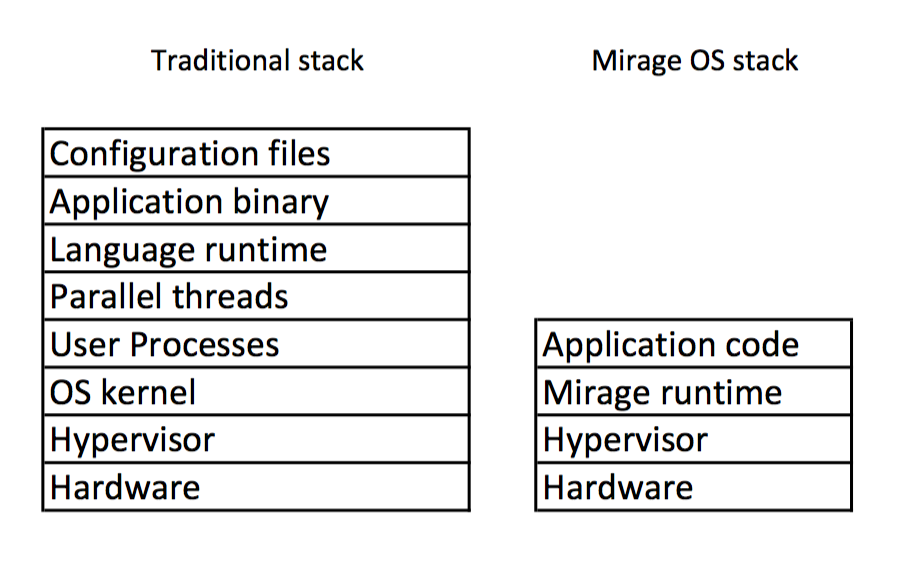
\includegraphics[width=0.5\textwidth]{images/design}
\end{figure}

The unikernel concept was first outlined .

Today there are server operating systems developed for cloud computing that based on the concept of unikernels. MirageOS is a library operating system written in Ocaml that is commonly used for constructing unikernels.

% key-value datastore background
(What are key-value stores for?) 

Redis, short for Remote Dictionary server, is a key-value store software that is commonly used in distributed systems on virtualized operating systems. It features (). However, this software is generally run atop a full operating system installation, which incurs a certain degree of overhead as discussed previously.  While the OSv operating system can support Redis, it does not function optimally.


\section{Design and Implementation}

<<<<<<< HEAD
For Keyvee we have the following goals:
\begin{itemize}
  \item Implement subset of Redis functionality in OCaml on top of the Mirage OS toolchain
  \item Make Keyvee as compatible to Redis as possible.
  \item Implement RESP, Redis's protocol specification, to allow interoperability with existing tools and libraries.
\end{itemize}

Here in this section we will talk about our implementation of Keyvee and how we try to accomplish these goals.

\subsection{Overview}

\begin{figure}[ht]
  \centering
  \caption{Supported commands}
  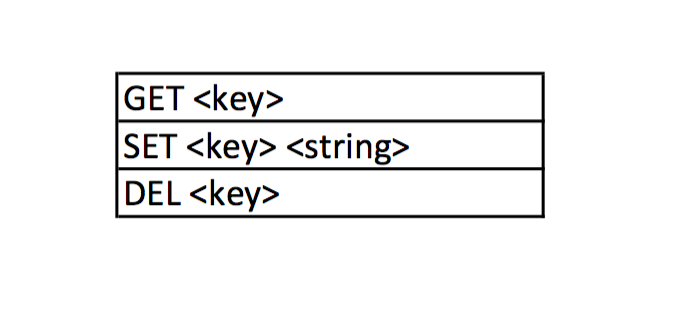
\includegraphics[width=0.5\textwidth]{images/commands}
\end{figure}

Keyvee is implemented on top of the Mirage OS toolchain using OCaml. Currently, we support the GET, SET and DEL commands. All data is stored in-memory, similar to Redis. We have an internal module implementation built on top of OCaml's Hashtbl module, which stores our keys and associated data in an efficient lookup table. We use a hash table with a seeded hash function, using a seed randomly chosen at hash table creation time. This means the hash function is randomly selected among 230 different hash functions with different collision patterns which helps stop denial-of-service attacks where attackers can send input crafted to create collisions, slowing our application to a halt.

We use MirageOS's low level TCP/IP network stack implemented in pure OCaml. Because memory layout in Mirage is used to distinguish I/O pages, the OCaml garbage collector needs to scan less to be as effective as in a full stack OS, which let's the network stack perform predictably. Predictable performance, as well as support for zero-copy I/O makes Mirage's network stack performant. The stack then hands off the raw data to our parse functions, which parse the data using string operations. The parse functions fully support well formed queries for our supported functions, but lack some verification steps and will not respond to badly formed queries. After the parse phase, the data is handed off to the Hashtbl module which responds with data or writes data. The response is then written to the client in RESP compatible format.

Mirage uses the Lwt, cooperative threading library, extensively and every request is wrapped in a lightweight cooperative thread. Leveraging Mirage and OCaml guarantees type safety in both our application as well as in the implementations of frameworks underlying the application such as the TCP/IP stack, enhancing the security of our implementation.

\subsection{Development process}

We use distributed version control system Git and Github to track changes to our codebase. Travis Continuous Integration is then used to build our codebase when changes are made and check for any errors. It is possible to build a Unix binary using the Mirage toolchain, which we use extensively when developing our code before it is deployed and tested on the Xen server. 

The Mirage OS documentation leaves a lot to be desired and a lot of times we needed to go looking into Mirage OS's implementation it self. In addition, some OCaml modules do not work with the toolchain and there is scarcity of open source code built with it. Especially as it is the early days there is not a lot of community support surrounding Mirage.


\section{Evaluation}
=======
The Mirage OS unikernel library operating system is leveraged to provide a correct and compact implementation. Mirage OS leverages the Ocaml language to provide type safety at a low level, this creates many guarantees in terms of correctness.
GET Operation
SET Operation
Evaluation
>>>>>>> origin/evaluation

To test the unikernel implementation, we utilized two of the benchmarking tools provided by the  ocam development kit. To get execution counts, the profiler “ocamlprof”, a part of the ocaml toolchain was used, inserting relevant information as comments to the code. To get detailed execution time information, the unikernel was compiled to include profiling information for the gprof tool.

Redis’ benchmarking tool was used to get data for comparison, running on both as a host system and a virtual machine. The Redis benchmarking tool was limited to four tests: inline ping, bulk ping, get method, and set method. For all tests, the benchmark made one million requests across fifty simulated parallel clients using a payload of three bytes.

The main point of comparison is the relative runtime of the unikernel implementation versus the two Redis setups. For each of the methods that were implemented
Collected Results

So far, the only benchmarks that have been completed were the Redis benchmarks for both the host-to-host setup and the native host setup. Preliminary benchmarks for the unikernel have been run.




<<<<<<< HEAD
\section{Related Work}

HaLVM\cite{halvm} and LING\cite{ling} are both alternatives to Mirage OS, using Haskell and Erlang respectively as the basis of their unikernel efforts. With all of these, you are limited to one functional language and the image is then built to run on top of the Xen hypervisor. Mirage OS and LING focuses on performance and predictability while HalVM focuses more on elegant compositional semantics using Haskell. Low level libraries are being implemented for the platforms in their native code, so while the work is ongoing the level of support varies. Mirage OS for example has a more mature SSL library and better support for encrypted connections then the other platforms.

OSv\cite{osv} is another variant to the special-purpose operating system using the library OS paradigm. In OSv everything runs in the kernel space and it's built to run as guest on top of a virtual machine. However, it contains necessary functionality to run Java and POSIX applications which allows OSv to run some existing codebases and get some of the performance benefit Mirage enjoys. Mirage however focuses on a toolkit to assemble new unikernel application without specific domain knowledge in kernel programming for example.

Arrakis\cite{arrakis}, SPIN\cite{spin} and Exokernel\cite{exokernel} all reduce shared kernel components and allow each application to have customized operating system management, achieving some of the increased performance benefit of Mirage OS without tying you to one language runtime.  Arrakis in particular benefits from increased support for virtualization in new hardware, which allows it to effectively run all applications in kernel space and achieve seperation using hardware instructions, similar to how Mirage OS achieves seperation through Xen.
=======

\section{Evaluation}

We performed all of our evaulations on a dedicated 8\-core HP ProLiant rack server with 16 GB RAM available.
Our Xen hypervisor installation is coordinated by a Ubuntu Server 14.04 host that serves as the management domain to manage the other hosts running on the Hypervisor.
The Mirage installation was modified to use Redis' communication protocols so that we could use the same benchmark for all test setups. The benchmark was run using 50 parallel clients sending a 3-byte payload. 
The Redis setups were given ten thousands requests as part of their benchmark, while the Mirage setups on Xen were given five hundred, one thousand, or ten thousand requests.


\subsection{Running Mirage}

When a Mirage OS unikernel is configured in Xen mode, both the unikernel image and the configuration file are generated.
With these, a unikernel can be easily launched using the xl Xen management tool.
Due to the small size of the image, this is a quick process where the Mirage image configures itself when started by xl.

\subsection{Network Overhead}

On examining the throughput and the completion times for requests between running the benchmark between two hosts, we found that there was a significant overhead imposed by network communications. For SET operations there was an increase of 42\% in execution time and GET operations saw a similar 43\% increase in execution time.
The benchmark results for the Mirage OS installation were found to have throughputs an order of magnitude lower than expected. 
Upon further testing and examination of code, it found that that the Mirage systems were not properly handling multiple simultaneous clients, resulting in a very low throughput which was noticed in further tests.


\subsection{Mirage \- UNIX}

Three different benchmarks setups were tested, making either five hundred, one thousand, or ten thousand total requests. 
Similarly to the tests run on the Mirage installations that were on top of Xen, the throughput was also an order of magnitude lower when compared to Redis. 
Strangely, the Unix-based setups did much better for the five hundred and one thousand request trials, but did extremely poorly for the ten thousand request setup.

\subsection{Throughput Performance}

\begin{figure*}[ht]
  \centering
  \caption{Average Throughputs}
  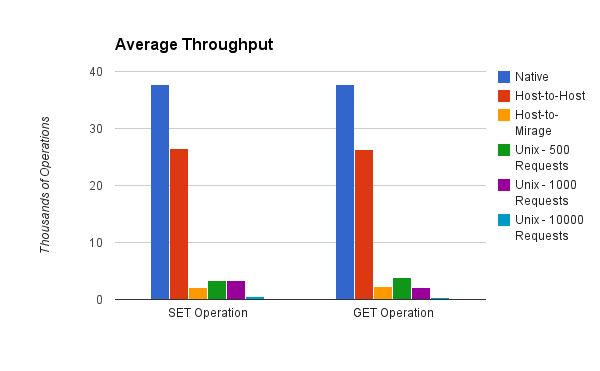
\includegraphics[width=1.0\textwidth]{images/throughput}
\end{figure*}

\begin{table}[h]
\begin{tabular}{lll}
Average Throughput & SET Operation & GET Operation \\
Native & 37766.142 & 37792.576 \\
Host-to-Host & 26571.512 & 26348.028 \\
Mirage on Xen & 2188.18 & 2222.22 \\
Unix (500) & 3401.36 & 3787.88 \\
Unix (1000) & 3344.48 & 2024.29 \\
Unix (10000) & 580.55 & 338.26
\end{tabular}
\caption{Average throughputs (requests per second)}
\label{my-label}
\end{table}

Overall, the Mirage systems showed markedly worse throughput performance, at a staggering order of magnitude lower than the baseline Redis benchmarks. 
Corrections to the Mirage coding are underway so that a fair benchmark comparison can be made and a provide a more representative view.

\section{Conclusion}
% @NATE


\section{Acknowledgements}
We thank the kind souls in the \#Mirage IRC chatroom for their relentless patience.
Their assistance was crucial in learning how to use Mirage's utilities and leverage the provided standard library.


>>>>>>> origin/evaluation


\bibliographystyle{abbrv}
\bibliography{bibliography}


\end{document}



